\documentclass{standalone}
\usepackage{tikz}
\usetikzlibrary{positioning}
\usetikzlibrary {matrix}
\usetikzlibrary {shapes.multipart}

\begin{document}
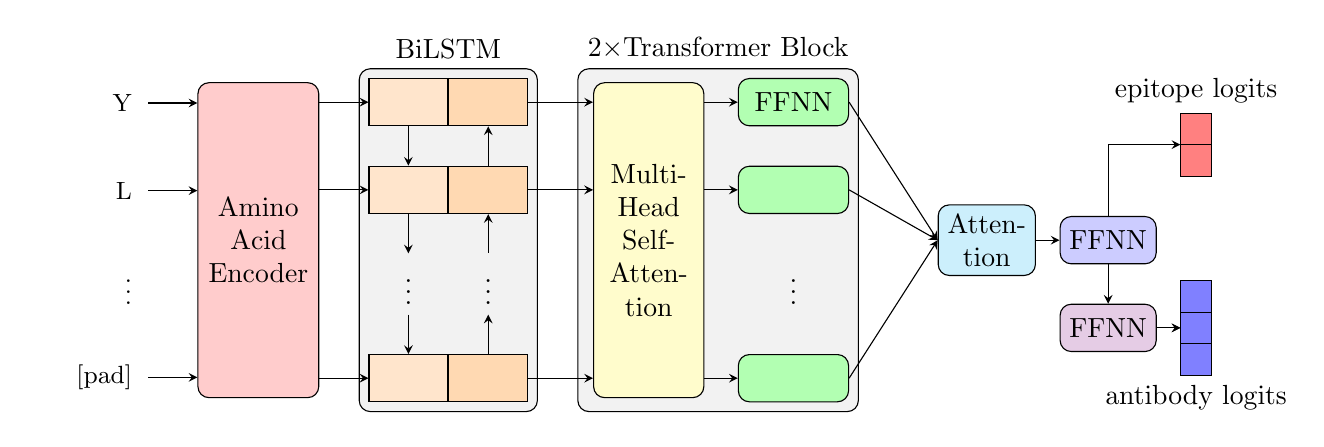
\begin{tikzpicture}
[
node distance=5mm and 5mm,
>=stealth,
box/.style={rounded corners, minimum height=6mm, anchor=center, draw},
bigbox/.style={rounded corners, minimum width=14mm, minimum height=40mm, align=center, draw},
vector/.style={rectangle split, rectangle split parts=#1, draw},
texts/.style={draw opacity=0, fill=none},
]

\matrix (input)
[
matrix of nodes,
nodes={box, minimum width=14mm, node font=\small, text width=10mm, align=right, draw opacity=0},
row sep=5mm,
] at (0,0)
{
Y \\
L \\
|[texts]|{$\vdots$} \\
{[pad]} \\
};
\node (enc) [bigbox, right=of input, text width=13mm, fill=red!20] {Amino Acid Encoder};

\matrix (lstm)
[
right=of enc,
matrix of nodes,
nodes={box, sharp corners, minimum width=10mm, draw},
column 1/.style={nodes={fill=orange!20}},
column 2/.style={nodes={fill=orange!30}},
nodes in empty cells,
row sep=5mm,
label=above:BiLSTM,
rounded corners,
draw,
fill=gray!10,
]
{
& \\
& \\
|[texts]|{$\vdots$} & |[texts]|{$\vdots$} \\
& \\
};

\matrix (te)
[
right=of lstm,
matrix of nodes,
nodes={box, minimum width=14mm, draw},
column 1/.style={nodes={draw opacity=0}},
column 2/.style={nodes={fill=green!30}},
nodes in empty cells,
row sep=5mm,
column sep=5mm,
label=above:2$\times$Transformer Block,
rounded corners,
draw,
fill=gray!10,
]
{
& FFNN \\
& \\
& |[texts]|{$\vdots$} \\
& \\
};

\node (mhsa) [bigbox, right=of lstm, xshift=2mm, text width=10mm, fill=yellow!20] {Multi-Head Self-Atten-tion};

\node (attn) [box, right=of te, xshift=5mm, text width=10mm, align=center, fill=cyan!20] {Atten-tion};
\node (ff1) [box, right=of attn, xshift=-2mm, fill=blue!20] {FFNN};
\node (ff2) [box, below =of ff1, fill=violet!20] {FFNN};
\node (out1) [vector=2, above right=of ff1, xshift=-2mm, label=above:epitope logits, fill=red!50] {};
\node (out2) [vector=3, right=of ff2, xshift=-2mm, label=below:antibody logits, fill=blue!50] {};

\foreach \i in {1,2,4}
{
\draw [->] (input-\i-1.east) -- (input-\i-1.east -| enc.west);
\draw [->] (enc.east |- lstm-\i-1.west) -- (lstm-\i-1.west);
\draw [->] (lstm-\i-2.east) -- (lstm-\i-2.east -| mhsa.west);
\draw [->] (mhsa.east |- te-\i-2.west) -- (te-\i-2.west);
\draw [->] (te-\i-2.east) -- (attn.west);
}
\foreach \x / \y in {1/2,2/3,3/4}
{
\draw [->] (lstm-\x-1) -- (lstm-\y-1);
\draw [<-] (lstm-\x-2) -- (lstm-\y-2);
}
\draw [->] (attn) -- (ff1);
\draw [->] (ff1) |- (out1);
\draw [->] (ff1) -- (ff2);
\draw [->] (ff2) -- (out2);
\draw [->] (ff2) -- (out2);
\end{tikzpicture}
\end{document}
